\chapter{Metodologia}
\label{cap:metodologia}

Para explorar a visualização dos fluxos de mobilidade urbana utilizamos em nosso
estudo dados públicos da pesquisa OD17. Esses dados representam milhões de viagens
que ocorrem diariamente em um dia normal de trabalho na Região Metropolitana
de São Paulo (RMSP). Parametrizamos e adaptamos o \emph{framework} de visualização \emph{CUBu} para explorar várias
propriedades do tráfego com diferentes usos do \emph{bundling}. A seguir
detalhamos cada uma das etapas que seguimos.

\section{Representação dos Dados}

Os dados da pesquisa OD que usamos como entrada para o \emph{bundling} são
descritos por uma tabela com 6 (seis) colunas: ID da viagem, modo de transporte,
horário de partida, horário de chegada, coordenadas de origem e coordenadas de
destino; O ID da viagem é o identificador obtido
diretamente do conjunto de dados da OD17 e representa uma entrada única no conjunto
de dados. O modo de transporte é armazenado como um número inteiro no intervalo
de 1 a 17 e corresponde a cada um dos diferentes modos presentes na pesquisa OD17.
Os horários de partida e chegada são armazenado como um número de ponto
flutuante no intervalo de [0.0 - 23:59]. Por último, temos as coordenadas de
origem e destino, o principal atributo do conjunto de dados. Em se tratando de
coordenadas, diversos sistemas podem ser utilizados; em nossa pesquisa
transformamos todas as coordenadas para o sistema de latitude / longitude para a
correta geo-localização das viagens no mapa, que também utiliza este formato.

Um outro atributo importante é o fator de expansão de cada registro da OD17 (apresentado na Seção~\ref{sec:pesquisa-od}),
o qual é utilizado para extrapolação estatística da quantidade real estimada de viagens.
Desta forma, dado o registro de uma viagem da pesquisa OD17 contendo um fator de expansão $E$, criamos $E$
cópias desse registro para utilizar como entrada da nossa visualização com \emph{bundling}. Isso produz um conjunto de dados completo de 42
milhões de viagens. Para todas essas viagens replicadas, mantemos seu ID original
obtido da pesquisa OD17 que a gerou. Dessa forma, podemos rastrear quais viagens
agrupadas correspondem a um registro da OD17. Além desses dados básicos que apresentamos, atributos
extras da pesquisa OD17 podem ser adicionados, como o motivo da viagem (ver
Seção~\ref{sec:pesquisa-od}) e também dados pessoais (idade, renda). A pesquisa
OD é bastante rica e pode produzir um conjunto de dados com mais de dez atributos por viagem.
A Tabela~\ref{table:data-input} mostra um exemplo das viagens geradas com duas
viagens replicadas a partir de um registro da OD com ID 50 e fator de expansão $E=2$.

% Using the siunitx package to align and round
% numbers (columns of type "S")
\begin{table}[!htb]
  \small
  \newcommand{\hdr}[1]{\bfseries#1}
  \sisetup{
    mode=text,
    round-mode=places,
    round-precision=6,
    table-figures-integer=2,
    table-figures-decimal=6,
    table-number-alignment=left,
    table-text-alignment=left,
    table-space-text-post=nn,
  }
  \centering
  \caption{Formato de dados utilizados como entrada para o \emph{bundling}.\label{table:data-input}}
  \begin{tabular}{>{\footnotesize}l>{\footnotesize}c>{\footnotesize}l>{\footnotesize}l>{\footnotesize}S>{\footnotesize}S>{\footnotesize}S>{\footnotesize}S}
    \toprule
    \multirow{2}[2]{*}{\hdr{ID}} & \multirow{2}[2]{*}{\hdr{Modo}} & \hdr{Saída} & \hdr{Chegada} & \multicolumn{2}{c}{\hdr{Origem}}   & \multicolumn{2}{c}{\hdr{Destino}}\\
     &  & \hdr{hora} & \hdr{hora} & \hdr{Longitude}   & \hdr{Latitude}    & \hdr{Longitude}     & \hdr{Latitude}\\
    \midrule
    50         & 1   & 6.45 & 7.10  & -46.62809376987491 & -23.551691865840347 & -47.00348104352116 & -23.39356328288028\\
    50         & 1   & 6.45 & 7.10  & -46.62809376987491 & -23.551691865840347 & -47.00348104352116 & -23.39356328288028\\
    51         & 4   & 8.30 & 9.05  & -47.00187231236886 & -23.39846860627696  & -47.00348104352116 & -23.39356328288028\\
    \bottomrule
  \end{tabular}
\end{table}

\section{Pré-processamento dos dados}

Como mencionado na Seção~\ref{sec:pesquisa-od}, o conjunto de dados possui \num{157992} viagens,
e que ao considerarmos o fator de expansão, esse número cresce para pouco mais de 42 milhões.
Embora \emph{CUBu} seja - de acordo com seus autores e também com nosso conhecimento - a
solução mais rápida existente para agrupamento com \emph{bundling}, ele ainda não
seria capaz de processar 42 milhões de viagens e responder de maneira rápida para
exploração interativa dos dados. Para lidar com este problema, utilizamos uma abordagem
para reduzir o conjunto de dados OD17 com base no fator de expansão $E$.

Primeiramente, analisamos quão representativos eram os registros amostrais da
OD17 em relação a população total de 42 milhões de viagens. Observamos que todos os
registros com fator de expansão $E < 75$, quando somados, representavam menos de 4\% da população total de 42
milhões. Considerando que a margem de erro da pesquisa OD17 é inferior a 6\%
(ver Seção~\ref{sec:pesquisa-od}), podemos remover os registros com $E < 75$ e
ainda assim manter a representatividade do conjunto de dados. Então, pudemos dividir
os valores $E$ de todos os registros restantes por esse valor limite de 75,
resultando em um número menor de viagens a serem duplicadas, e ainda preservar
a distribuição de dados. No entanto, embora 75 seja um valor dentro de um
limite razoável para aplicar a redução, conforme explicado acima, para minimizar
a perda de dados e evitar grandes alterações nas suas propriedades, nós
utilizamos na prática um limite menos agressivo de 55. A
Figura~\ref{fig:expansion-factor} mostra o percentual acumulado de registros que
são removidos pela escolha de determinados valores do fator de expansão, quanto
maior o valor, mais dados são perdidos na redução. Essa abordagem nos permitiu
reduzir significativamente o número de viagens, de 42 milhões para \num{685115},
o que resultou em menos de 2,5\% de perda de informações.

\begin{figure}
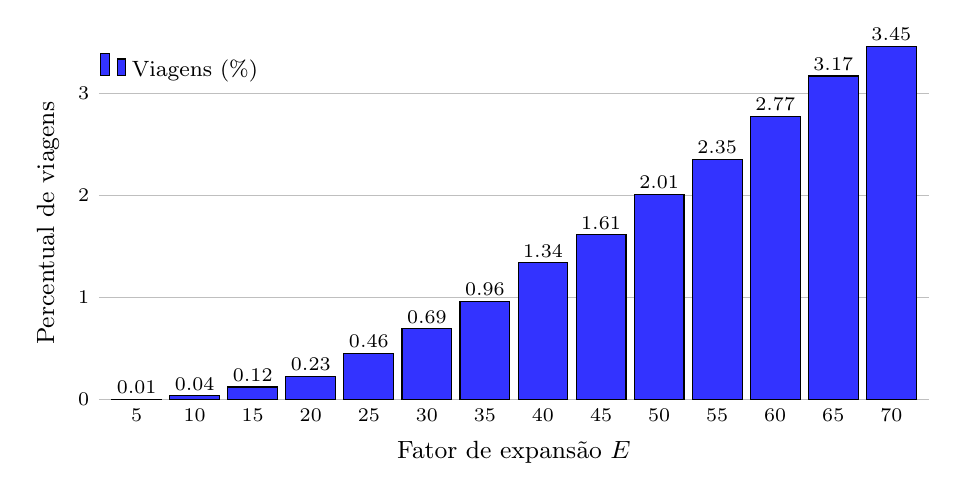
\begin{tikzpicture}
  \begin{axis}[
    ybar=0pt,
    bar width=18pt,
    bar shift = 0pt,
    width=\textwidth,
    height=0.5\textwidth,
    tickwidth         = 0pt,
    enlarge y limits  = 0,
    enlarge x limits  = 0.05,
    symbolic x coords = {5,10,15,20,25,30,35,40,45,50,55,60,65,70},
    xtick = data,
    ylabel near ticks,
    ylabel={Percentual de viagens},
    xlabel={Fator de expansão $E$},
    ymin=0,
    ymajorgrids,
    y axis line style = { opacity = 0 },
    label style={font=\small},
    tick label style={font=\scriptsize},
    nodes near coords,
    every node near coord/.append style={font=\scriptsize,color=black,yshift=0.25cm,rotate=0,anchor=north,inner sep=0.3pt,/pgf/number format/fixed},
    legend style={at={(0.1,1.0)},anchor=north,legend columns=-1,font=\footnotesize,draw=none},
  ]
  \addplot[fill=blue!80] coordinates {(5,0.0052)(10,0.0363)(15,0.1235)(20,0.2258)(25,0.4561)(30,0.6931)(35,0.9593)(40,1.3396)(45,1.6128)(50,2.0119)(55,2.3489)(60,2.7709)(65,3.1686)(70,3.4546)};
  \legend{Viagens ($\%$)}
  \end{axis}
\end{tikzpicture}
\caption{Percentual acumulado da perda de registros em função do fator de expansão.}
\label{fig:expansion-factor}
\end{figure}

\section{Filtragem e particionamento dos dados}

Além do processo de redução de dados explicado acima, também aplicamos dois
outros métodos de simplificação, \emph{filtragem} e \emph{particionamento}. Tais
técnicas permitem um outro olhar para características específicas do conjunto de
dados e funcionam de maneira complementar. Com as duas abordagens,
exploramos duas diferentes utilizações do \emph{bundling}, o que permitiu uma
experiência maior para avaliar o potencial da técnica na análise
de grandes conjuntos de dados de mobilidade urbana com múltiplos atributos.

Para ver as relações entre os diferentes modos de transporte e as direções do
tráfego durante os horários de pico, usamos filtros visuais que tornam as
trajetórias indesejadas totalmente transparentes na visualização. Isso é
particularmente útil quando queremos visualizar relações entre dados diferentes,
por exemplo, para explorar como os ônibus de São Paulo se relacionam com os
ônibus de outras cidades vizinhas. Nesse caso, aplicar \emph{bundling} em todo o
conjunto de dados e, em seguida, diferenciá-los de alguma forma na visualização,
é uma maneira sugestiva de visualizar suas relações. A diferenciação pode ser
feita de várias formas, e aqui utilizamos cores diferentes para cada tipo de
transporte e opções de filtro diferentes, os quais abordaremos adiante.

Para outros tipos de análises, como as relacionadas ao motivo da viagem, renda
familiar e idade dos passageiros, nós particionamos o conjunto de dados em cada
um desses atributos separadamente e aplicamos o \emph{bundling} a esses
subconjuntos. As vantagens dessa abordagem é que ela permite observar cada
atributo com mais detalhes, pois remove a interferência de outros dados, além de
ser mais simples de se executar.

\section{Parâmetros do \emph{bundling}}

Referências da literatura não são claras sobre como escolher bons parâmetros de
\emph{bundling}, \cite{Lhuillier2017}. Isso também foi observado e explicitamente
estudado por \cite{zeng:19}, que também propôs maneiras de calcular boas
configurações de parâmetros. No entanto, como eles também mencionam, essas
configurações são válidas para seu método de \emph{bundling} (RAEB) e não
generalizam diretamente para outros métodos, como o \emph{CUBu}. Portanto,
tivemos que encontrar bons parâmetros para nosso estudo empiricamente. Os
parâmetros obtidos dessa forma foram: resolução da imagem $I = 512 x 512$
pixels; taxa de preenchimento $S = 10$ pixels (de acordo com a recomendação de
\cite{zwan:16} de usar 1\% da diagonal da imagem); raio do kernel $k = 18$
pixels; e número de iterações do \emph{bundling} $N = 15$. Em nosso maior
conjunto de dados, representado por todas as \num{685115} viagens, esta
configuração gerou cerca de 3,2 milhões de pontos, que foram agrupados em cerca
de 52 milissegundos por iteração em um PC com uma placa de vídeo NVidia GeForce
940MX de 4 GB. Usamos esse conjunto de parâmetros para criar a maioria das
visualizações agrupadas mostradas a seguir na Seção~\ref{sec:results}, exceto para as da Seção~\ref{sec:classes},
onde mostramos os padrões de deslocamento de diferentes classes sociais.
Para esses subconjuntos específicos, reduzimos a taxa de preenchimento $S$ para
5 pixels e modulamos a transparência $alpha$ do mapa de densidade para 0,15. Na
prática, ao utilizarmos metade do valor de $S$ dobramos o número de pontos na
visualização;  Observamos que as mudanças desse dois parâmetros ajudam a
destacar os pontos de densidade que buscamos em nossa análise sem impacto na
estrutura da visualização.

% TODO arrumar referencias das seções 5 e 5.6 no paragrafo anterior

\section{Melhorias na visualização}

Para enriquecer nossas visualizações da mobilidade urbana de São Paulo, fizemos
algumas importantes adições ao \emph{CUBu}. Primeiro, adicionamos o mapa da área
metropolitana como imagem de fundo e também a possibilidade de desenhar as
linhas de metrô e trem na visualização. Dessa forma, podemos utilizar o mapa
para localizar melhor onde os \emph{bundles} estão posicionados e podemos usar
os trilhos para explorar como os \emph{bundles} se correspondem com a
infraestrutura ferroviária da cidade (ver Seção~\ref{sec:trail-overlap}). Além
disso, implementamos filtros para selecionar subconjuntos dos 17 modos de
transporte a serem exibidos na visualização, usando cores categóricas diferentes
para cada um deles (ver Seção~\ref{sec:coloring} e filtros de tempo para selecionar fluxos de movimentação em
horários específicos do dia (ver Seção~\ref{sec:peak-hours}). Usamos esses recursos para explorar a diferentes
relações entre os fluxos e seu impacto na mobilidade urbana.
